\documentclass[tikz,border=2pt]{standalone}
\usepackage{amsmath,amssymb}
\usetikzlibrary{arrows.meta}

\begin{document}
% Rectangles [n, n+1] x [0, 1/n] for n = 1, ..., 6 lie above y = 1/x on [n, n+1]; their areas are
% 1, 1/2, 1/3, ..., so the partial sums of sum 1/n dominate the integral of 1/x from 1.
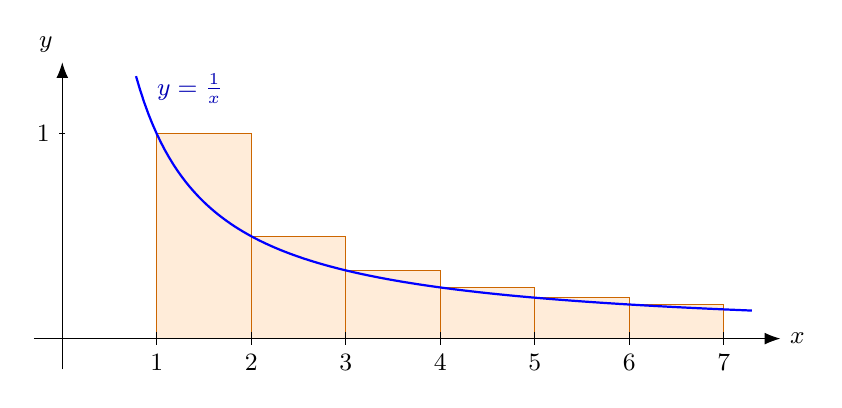
\begin{tikzpicture}[every node/.style={font=\small}, >={Latex[length=2mm]}, x=1.2cm, y=2.6cm]
	\foreach \n in {1,...,6} {
		\filldraw[fill=orange!15, draw=orange!80!black] (\n,0) rectangle ({\n+1},{1/\n});
	}
	\draw[->] (-0.3,0) -- (7.6,0) node[right] {$x$};
	\draw[->] (0,-0.15) -- (0,1.35) node[above left] {$y$};
	\foreach \x in {1,...,7} {
		\draw (\x,0.03) -- (\x,-0.03) node[below, font=\small] {$\x$};
	}
	\draw (0.03,1) -- (-0.03,1) node[left, font=\small] {$1$};
	\draw[blue, thick, domain=0.78:7.3, samples=150] plot (\x,{1/\x});
	\node[blue!70!black, anchor=west] at (0.9,1.22) {$y=\frac1x$};
\end{tikzpicture}
\end{document}
